% =============================================================================
% FIRE 2026 — Regular Paper (DOUBLE-BLIND) — REVISED
% ACM ICPS, sigconf, two columns. Maximum 9 pages of content, references excluded.
%
% Anonymity: no author names, no affiliation, no repository URL that identifies
% the authors. Concrete artifact locations are restored in the camera-ready.
% =============================================================================
\documentclass[sigconf,natbib=true,anonymous=true]{acmart}

\AtBeginDocument{%
  \providecommand\BibTeX{{\normalfont B\kern-0.5em{\scshape i\kern-0.25em b}\kern-0.8em\TeX}}}

\setcopyright{none}
\settopmatter{printacmref=false}
\renewcommand\footnotetextcopyrightpermission[1]{}
\pagestyle{plain}
\acmConference[FIRE 2026]{Forum for Information Retrieval Evaluation}{December
  2026}{India}

\usepackage{booktabs}
\usepackage{adjustbox}
\usepackage{graphicx}
\usepackage{amsmath}

\begin{document}

\title{Single-Point Bias Comparisons Are Fragile: An Iso-Loss Sensitivity Study
       of Weight-Shared Transformer Encoders}

\author{Anonymous Author(s)}

% ------------------------------------------------------------------- abstract
\begin{abstract}
Comparing the social bias of two neural architectures is confounded by
capability: a better-trained model gives sharper answers on every probe, so a
difference measured after a fixed training budget mixes architecture with
training progress. The usual remedy is to compare checkpoints matched on
validation loss, and this study asks how far that comparison can be trusted.
Four encoders differing in how weights are reused across depth were
pre-trained on identical data, snapshotted at matched validation loss, and scored
on a paired stereotype benchmark of 1508 items. At the deepest matched point two
of the three weight-shared encoders record a lower stereotype effect than the
unshared baseline, and both differences survive correction. That result does not
generalise. Recomputed at every distinct matched point the contrast changes sign,
and the point supporting the reduction is the only one of five where the looped
encoder falls below the baseline. Adjusting continuously for realised loss leaves
no architecture difference distinguishable from zero while the loss term remains
clearly non-zero. Substituting the changed-token scoring rule used by the
benchmark's own implementation removes every architecture difference after
correction, and the two rules agree only moderately at item level. Aggregate
scores further conceal sign changes across bias categories. All four encoders
answer at chance on a coreference instrument, so these measurements index
association in the masked language modelling head, not downstream behaviour. Architecture fairness comparisons should therefore report sensitivity
across capability levels and scoring rules rather than a single matched
operating point.
\end{abstract}

% ---------------------------------------------------------- CCS and keywords
\begin{CCSXML}
<ccs2012>
<concept>
<concept_id>10010147.10010178.10010179</concept_id>
<concept_desc>Computing methodologies~Natural language processing</concept_desc>
<concept_significance>500</concept_significance>
</concept>
<concept>
<concept_id>10002951.10003317.10003338</concept_id>
<concept_desc>Information systems~Retrieval models and ranking</concept_desc>
<concept_significance>300</concept_significance>
</concept>
<concept>
<concept_id>10003456.10010927</concept_id>
<concept_desc>Social and professional topics~User characteristics</concept_desc>
<concept_significance>300</concept_significance>
</concept>
</ccs2012>
\end{CCSXML}

\ccsdesc[500]{Computing methodologies~Natural language processing}
\ccsdesc[300]{Information systems~Retrieval models and ranking}
\ccsdesc[300]{Social and professional topics~User characteristics}

\keywords{social bias, masked language models, parameter sharing, evaluation
robustness, iso-loss comparison, fairness measurement}

\maketitle

% =============================================================== introduction
\section{Introduction}

Pre-trained encoders sit underneath much of current retrieval and text
classification practice. One masked language model is trained and then reused
across rankers, classifiers and filters, so a stereotypical association acquired
during pre-training is inherited by every component built on it. Practitioners
therefore have a reason to ask whether one architecture carries less of that
association than another.

The question is harder to answer than it looks. Two architectures with the same
parameter count do not reach the same language modelling quality, and a model
further along in training assigns sharper probabilities to every probe, including
the minimal pairs used by stereotype benchmarks. A difference measured after a
fixed number of training tokens therefore mixes the architecture with how well
each model has learned the language. Studies of compression and fairness report
mixed and sometimes opposing outcomes
\citep{hooker2020characterising,xu2022compression,ramesh2023comparative}, and
they do not control this confound directly.

Matching checkpoints on validation loss is the natural remedy, and it is the
design used here: each encoder is trained until its validation loss crosses a
list of values fixed before training, and a snapshot is written at each crossing.
This paper takes that design seriously enough to test it. Matching removes gross
differences in training progress, but it leaves two choices that are rarely
examined: \emph{which} matched capability level to report, and \emph{which}
scoring formulation to apply to the benchmark. Both turn out to matter more than
the architecture.

Four encoders are compared, differing only in how weights are reused across
depth: an unshared baseline, a looped encoder that applies six blocks twice, an
ALBERT-style encoder that applies one block twelve times \citep{lan2020albert},
and a looped encoder extended with four parallel residual streams joined by
hyper-connections \citep{zhu2025hyperconnections}. Three of the four share
weights across depth, so any statement about ``shared'' encoders has to account
for all three.

This paper makes four contributions.

\begin{enumerate}
\item An iso-loss robustness protocol that separates architecture comparisons
      from gross training-progress differences and then tests explicitly whether
      a conclusion survives the choice of matched capability level and of scoring
      formulation.
\item Evidence that the apparent architecture effect on this benchmark is
      sensitive to both choices. It reverses sign across matched-loss points, and
      it does not survive correction under the benchmark's own changed-token
      scoring formulation.
\item An exploratory equivalence result placing the two looped variants within a
      margin of one another, so the additional routing mechanism shows no
      measurable association benefit under the conditions tested.
\item Evidence that an aggregate stereotype score conceals sign changes at the
      level of individual bias categories, together with a capability-gate result
      showing that these measurements should not be read as downstream
      behavioural fairness at this training scale.
\end{enumerate}

Section~\ref{sec:related} reviews the relevant measurement and weight-sharing
literature. Section~\ref{sec:method} defines the encoders, the matching protocol
and the two scoring formulations. Section~\ref{sec:results} reports the
robustness analyses, and Section~\ref{sec:limits} states what the evidence does
not support.

% ================================================================ related work
\section{Related Work}
\label{sec:related}

\paragraph{Measuring stereotype association in masked models.}
CrowS-Pairs scores a model on minimal pairs differing only in a demographic term
and records how often the stereotypical member receives the higher
pseudo-log-likelihood \citep{nangia2020crows}. StereoSet uses a related paired
construction \citep{nadeem2021stereoset}, building on the masked-position probing
of \citet{kurita2019measuring}. The instruments carry documented problems.
\citet{blodgett2021salmon} audited them and found unclear or inconsistent items
in a large share of pairs, warning against reading one aggregate number as a
measure of harm. \citet{wang2025difference} separate correlation-type benchmarks,
which record association, from descriptive and normative benchmarks, which record
whether a model treats groups differently when it should. The measure used here
is of the correlation type.

\paragraph{Weight sharing and looped depth.}
ALBERT ties one encoder block across all layers and trades quality for storage
\citep{lan2020albert}. \citet{saunshi2025looped} show that a $k$-layer block
looped $L$ times approaches the reasoning performance of a $kL$-layer model, and
\citet{bae2025mor} learn a per-token recursion depth over a shared block.
\citet{geiping2025huginn}, \citet{zhu2025ouro} and \citet{frey2026adaptive} study
related recurrent-depth models. Hyper-connections generalise the residual
connection to several parallel streams with learned mixing
\citep{zhu2025hyperconnections}, later constrained to a manifold by
\citet{xie2025mhc}; \citet{zeitoun2026hyperloop} combine looping with
hyper-connections. This literature evaluates quality, efficiency and reasoning,
not social bias.

\paragraph{Capacity, compression and fairness.}
\citet{hooker2020characterising} found that pruning degrades accuracy unevenly
across groups. \citet{xu2022compression} and \citet{ramesh2023comparative} report
outcomes whose direction depends on the compression method and the benchmark,
and \citet{voria2026tracing} localise stereotype-carrying neurons inside
pre-trained transformers. These studies compress a model after training. The
present work varies sharing before training and compares at matched quality,
which isolates the architectural question from the recovery dynamics of a
compressed checkpoint. The disagreement among their conclusions is itself part of
the motivation: if the measured direction depends on evaluation choices, mixed
results across studies are expected.

\paragraph{Robustness of fairness measurement.}
Fairness in information access is an established concern for retrieval and
ranking systems \citep{ekstrand2022fairness,singh2018fairness}. The present study
contributes to the measurement side of that literature rather than to ranking
itself: it asks whether a comparison between two encoders is stable under
defensible variations of the evaluation procedure.

% ===================================================================== method
\section{Method}
\label{sec:method}

\subsection{Architectures}

All four encoders use hidden size 768, twelve effective depths, one tokeniser and
the same masked language modelling objective \citep{devlin2019bert}, and differ
only in weight reuse across depth. \emph{VanillaBERT} holds twelve independent
blocks and is the unshared control. \emph{LoopedBERT} holds six blocks and
applies the stack twice. \emph{ALBERTLoopedBERT} holds one block and applies it
twelve times \citep{lan2020albert}. \emph{HyperloopBERT} keeps the six-block loop
and adds four parallel residual streams joined by hyper-connections
\citep{zhu2025hyperconnections}: instead of a single residual path the model
carries $n$ streams and mixes them at each depth,
%
\begin{equation}
\mathbf{H}^{(\ell+1)} = \mathbf{A}^{(\ell)}\mathbf{H}^{(\ell)}
                      + \mathbf{B}^{(\ell)} f\!\left(\mathbf{H}^{(\ell)}\right),
\end{equation}
%
where $\mathbf{H}^{(\ell)} \in \mathbb{R}^{n \times d}$ stacks the $n$ stream
states of width $d$ at depth $\ell$, $f$ is the shared transformer block,
$\mathbf{A}^{(\ell)} \in \mathbb{R}^{n \times n}$ mixes the streams and
$\mathbf{B}^{(\ell)} \in \mathbb{R}^{n \times n}$ distributes the block output
back across them; $n=1$ with $\mathbf{A}=\mathbf{B}=1$ recovers the ordinary
residual connection. Relative to the hyper-connected looped transformer of
\citet{zeitoun2026hyperloop}, this implementation shares the loop-and-stream
structure and the learned depth-wise mixing, and differs in being trained from
scratch at encoder scale under a masked language modelling objective. The
negative result below therefore concerns this configuration of the mechanism, not
every possible realisation of it. Table~\ref{tab:arch} gives the sizes.

\begin{table}[t]
\centering
\caption{The four encoders. All use hidden size 768 and twelve effective depths,
and differ only in weight reuse across depth.}
\label{tab:arch}
\small
\begin{adjustbox}{max width=\columnwidth}
\begin{tabular}{lccc}
\toprule
Architecture & Unique blocks & Parameters & Shared ratio \\
\midrule
VanillaBERT       & 12 & 110.1\,M & 0.00 \\
LoopedBERT        &  6 &  67.6\,M & 0.50 \\
HyperloopBERT     &  6 &  86.5\,M & 0.50 \\
ALBERTLoopedBERT  &  1 &  32.1\,M & 0.92 \\
\bottomrule
\end{tabular}
\end{adjustbox}
\end{table}

\subsection{Iso-loss matching and its limits}

A list of target validation loss values is fixed before training. Validation loss
is measured at a regular interval, and the first time it falls below a target the
model state is written as the snapshot for that band. Encoders are compared only
at snapshots carrying the same band.

Two properties of this procedure govern the analysis. First, several nominal
bands are sometimes crossed inside one validation interval, so they share a
single snapshot; treating them as separate observations would inflate the
apparent number of measurements. The analysis therefore works with
\emph{distinct} snapshots, which reduces seven nominal bands to between four and
seven distinct comparisons depending on the encoder. Second, matching is
approximate: a snapshot is taken at the first measurement below the target, so
realised losses differ slightly between encoders at the same band. Iso-loss
matching reduces training-progress confounding; it does not eliminate residual
capability differences, and Section~\ref{sec:cont} tests what remains.

\subsection{Two scoring formulations}

Each item is a pair of sentences differing only in a demographic term, one
stereotypical and one anti-stereotypical \citep{nangia2020crows}. Both
formulations below are pseudo-log-likelihoods computed in 32-bit precision by
masking one position at a time,
%
\begin{equation}
\mathrm{PLL}(s) = \sum_{i \in \mathcal{I}} \log P\!\left(t_i \mid s_{\setminus i}\right),
\end{equation}
%
where $s_{\setminus i}$ is the sentence with position $i$ masked and $P$ is the
masked language modelling head output. They differ in the index set
$\mathcal{I}$.

The \emph{full-sentence} formulation sums over all positions and normalises by
length, giving the per-item score
%
\begin{equation}
e = \bigl(\mathrm{PLL}(s_{\text{stereo}}) - \mathrm{PLL}(s_{\text{anti}})\bigr) / T .
\end{equation}
%
The \emph{changed-token} formulation, used by the reference implementation
released with the benchmark, restricts $\mathcal{I}$ to the tokens that differ
between the two members, so that shared context contributes nothing. Neither is
treated here as the correct scorer; they encode different assumptions about what
part of the sentence carries the association, and the empirical question is
whether a conclusion depends on that choice.

Architectures are contrasted item by item, so each pair yields one paired
difference. The test is a two-sided sign-flip permutation test with $10^4$ draws
and $p$-values computed as $(b+1)/(m+1)$ \citep{phipson2010permutation};
intervals are $10^4$-resample percentile bootstraps over items; Cohen's $d$ uses
the standard deviation of the paired differences. Corrections are Holm over the
three baseline-versus-shared contrasts.

\subsection{Capability gate}
\label{sec:gate}

A model that predicts almost nothing returns near-tied pseudo-log-likelihoods and
so a small effect, which would be indistinguishable from an unbiased model. Three
conditions were stated in advance for a bias reading to be interpretable: above-chance
GLUE performance \citep{wang2018glue}; a baseline effect interval excluding zero;
and above-chance accuracy on the pro-stereotype split of a coreference instrument
\citep{zhao2018winobias}, which tests whether the model resolves the pronoun at
all.

% ====================================================================== setup
\section{Experimental Setup}
\label{sec:setup}

All four encoders are pre-trained on the same corpus, 7 billion tokens of
FineWeb-Edu \citep{penedo2024fineweb} at sequence length 128, with one tokeniser
fitted once and reused, so no encoder sees different data or segmentation. The
corpus is pre-tokenised into fixed-size blocks and stored as a memory-mapped
array, and an integrity check compares the tokeniser checksum and block count
against a manifest at the start of every run. Training uses AdamW at a peak
learning rate of $3 \times 10^{-4}$, batch size 512, warmup over a tenth of the
steps, gradient clipping at 1.0, and bfloat16 autocast with FlashAttention
\citep{dao2022flashattention} on one H100 GPU. Encoders reach the deepest common
matched point after different token counts, between 1.53 and 2.07 billion.

HyperloopBERT is the one exception to the shared learning rate. At
$3 \times 10^{-4}$ its loss became non-finite, and at half that value it did so
later in training; its snapshots come from the run at $1.5 \times 10^{-4}$.
Holding the learning rate fixed would have compared three stable models against
one that failed to train, so the peak learning rate is tuned per architecture and
the arms are matched on validation loss rather than on hyper-parameters.

Training uses a single seed. Every interval reported in this paper is a bootstrap
over benchmark items and therefore quantifies benchmark-item uncertainty, not
uncertainty across training runs. No claim in this paper is supported by
replication across seeds.

% ==================================================================== results
\section{Results}
\label{sec:results}

\subsection{Quality and the matched points}

Validation loss over training appears in Figure~\ref{fig:training}.
VanillaBERT and LoopedBERT track each other closely for most of training,
while ALBERTLoopedBERT remains above both, so at this scale the six-block loop is
not under the capacity pressure that the single-block encoder is. HyperloopBERT
leaves the early plateau, where the model predicts little beyond token frequency,
after roughly half a billion tokens rather than the 1.4 billion the unshared arms
need; the same run later becomes non-finite. Section~\ref{sec:stability} treats
those events as observations about these runs, not as architecture properties.

\begin{figure}[t]
\centering
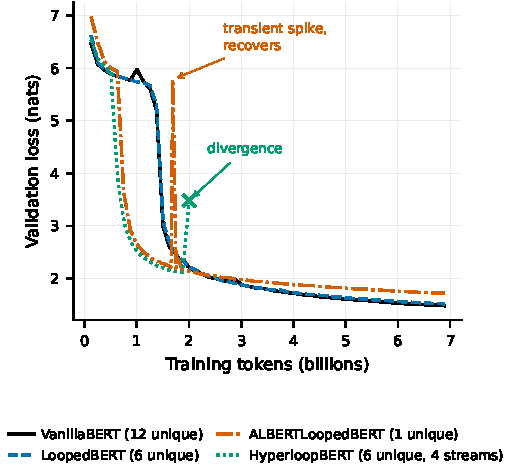
\includegraphics[width=\columnwidth]{images/fig2_training_dynamics.pdf}
\Description{Validation loss plotted against training tokens for four encoders.
HyperloopBERT descends earliest and its curve ends in a divergence marker near
two billion tokens. ALBERTLoopedBERT shows one spike that returns to trend.
VanillaBERT and LoopedBERT overlap closely and end lowest.}
\caption{Validation loss against training tokens. HyperloopBERT leaves the
plateau earliest and its run later diverges; ALBERTLoopedBERT shows one transient
spike that recovers.}
\label{fig:training}
\end{figure}

\subsection{The single matched point}

Table~\ref{tab:band} reports the deepest common matched point, where the four
snapshots agree to within 0.034 nats. Read alone, this table supports the
conclusion that weight sharing goes with a lower stereotype effect: LoopedBERT
and HyperloopBERT both sit below the baseline, and both contrasts survive Holm
correction with $p_{\text{Holm}} = 0.0003$. The third shared encoder does not:
ALBERTLoopedBERT differs by 0.0116 with an interval spanning zero
($p_{\text{Holm}} = 0.065$). The paired effects are small, near a tenth of a
standard deviation. The table also gives the benchmark's conventional stereotype
score, which places all four encoders between 55.4 and 55.8 and therefore
separates them far less than the effect-size column does.

\begin{table}[t]
\centering
\caption{Deepest common matched point. Snapshots agree within 0.034 nats.
Intervals are item bootstraps over 1508 pairs. $\Delta$ and $p_{\text{Holm}}$ are
against VanillaBERT.}
\label{tab:band}
\footnotesize
\begin{adjustbox}{max width=\columnwidth}
\begin{tabular}{lccccc}
\toprule
Architecture & Loss & Effect & 95\% interval & $\Delta$ & $p_{\text{Holm}}$ \\
\midrule
VanillaBERT      & 2.183 & 0.0707 & [0.045, 0.097] & --- & --- \\
LoopedBERT       & 2.192 & 0.0471 & [0.022, 0.072] & 0.0237 & 0.0003 \\
ALBERTLoopedBERT & 2.163 & 0.0591 & [0.034, 0.085] & 0.0116 & 0.0653 \\
HyperloopBERT    & 2.196 & 0.0466 & [0.022, 0.071] & 0.0241 & 0.0003 \\
\bottomrule
\end{tabular}
\end{adjustbox}
\end{table}

\subsection{The contrast does not hold across matched points}
\label{sec:allband}

Every encoder was snapshotted at several matched points, so the comparison in
Table~\ref{tab:band} can be repeated at each of them. Figure~\ref{fig:delta}
shows the result. The contrast crosses zero repeatedly. For the
baseline-versus-looped comparison, five distinct matched points are available and
the reduction reported in Table~\ref{tab:band} appears at exactly one of them;
at the four others the looped encoder records the \emph{higher} effect, and at
the matched pair 2.997 versus 2.968 nats — a tighter match than the headline
point — the difference is $-0.0222$ with $p = 0.0002$, significant in the
opposite direction. Averaged over its five matched points the contrast is
$-0.0063$. The comparisons against ALBERTLoopedBERT and HyperloopBERT are
positive at five of five and five of seven points respectively, but reach $p<0.05$
at only one and two of them.

\begin{figure}[t]
\centering
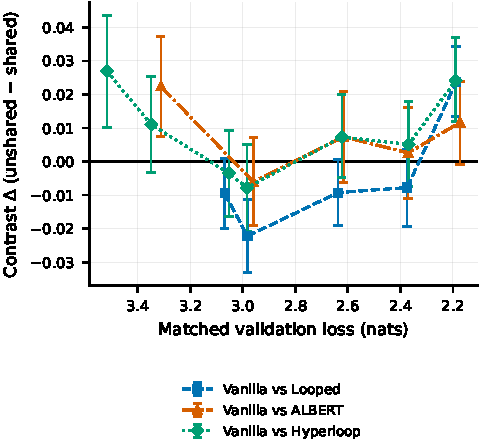
\includegraphics[width=\columnwidth]{images/fig3_delta_across_loss.pdf}
\Description{Architecture contrast plotted against matched validation loss with
bootstrap error bars. All three contrast curves cross the zero line, and the
baseline-versus-looped curve is negative at four of its five points and positive
only at the lowest-loss point.}
\caption{Architecture contrast against matched validation loss, which decreases
left to right as training progresses. Bands resolving to the same snapshot are
collapsed. The contrast changes sign across matched points, so the value at any
single point is not representative.}
\label{fig:delta}
\end{figure}

\subsection{Adjusting continuously for capability}
\label{sec:cont}

Matching at a band is a coarse control. Because the same 1508 items are scored
under every architecture at every snapshot, realised loss can instead be adjusted
for continuously. Pooling all 31\,668 architecture-snapshot-item observations
across 21 distinct snapshots, a linear model with architecture and realised loss
as predictors and standard errors clustered on benchmark item gives the estimates
in Table~\ref{tab:model}. No architecture differs from the baseline at the 5\%
level once realised loss is in the model, while the loss coefficient itself is
clearly non-zero: an encoder one nat further along records an effect larger by
about 0.018. The variance explained is very small, as expected when item-level
variation dominates.

Adding an architecture-by-loss interaction does not improve the model as a block
($p = 0.39$), though the looped interaction term is individually non-zero, which
is consistent with the sign change in Figure~\ref{fig:delta}. With four
architectures and between four and seven snapshots each there is too little
between-group structure to fit random slopes reliably, so a mixed model was not
attempted and this clustered estimate is reported instead.

\begin{table}[t]
\centering
\caption{Effect regressed on architecture and realised validation loss, standard
errors clustered on benchmark item. Baseline is VanillaBERT; loss is centred.
$n = 31\,668$ observations, 1508 items, 21 snapshots.}
\label{tab:model}
\footnotesize
\begin{adjustbox}{max width=\columnwidth}
\begin{tabular}{lccc}
\toprule
Term & Coefficient & 95\% interval & $p$ \\
\midrule
LoopedBERT        & $+0.0047$ & $[-0.0019,\ 0.0114]$ & 0.164 \\
ALBERTLoopedBERT  & $-0.0065$ & $[-0.0151,\ 0.0021]$ & 0.137 \\
HyperloopBERT     & $-0.0066$ & $[-0.0153,\ 0.0022]$ & 0.141 \\
Realised loss     & $-0.0184$ & $[-0.0291, -0.0076]$ & \textbf{0.0008} \\
\bottomrule
\end{tabular}
\end{adjustbox}
\end{table}

\subsection{Sensitivity to the scoring formulation}
\label{sec:scorer}

Both scoring formulations were computed for every item, so the contrast can be
recomputed without any new inference. Figure~\ref{fig:robust}(a) places them side
by side at the matched point. Under the changed-token formulation no contrast
survives Holm correction. The difference against the looped encoder falls from
0.0237 to 0.0054 ($p_{\text{Holm}} = 0.73$), that against ALBERT to 0.0062
($p_{\text{Holm}} = 0.73$), and baseline-versus-Hyperloop to 0.0143
($p_{\text{Holm}} = 0.063$). Item-level rank agreement between the formulations
is only $\rho \approx 0.46$--$0.49$, so they order individual pairs differently
rather than merely rescaling one another.

The changed-token formulation could not align 8 of the 1508 pairs. Inspection
shows why: those pairs differ in more than the demographic term — four to nine
words differ, and five of the eight have different lengths, as in \emph{``Whites
are not good at reading.''} against \emph{``Hispanics are good at reading''},
where the negation also changes. These are instances of the item-quality problem
documented by \citet{blodgett2021salmon}. Dropping them and imputing them from
the full-sentence formulation change the contrasts by less than 0.0006, so the
conclusion of this subsection does not rest on their treatment.

\begin{figure*}[t]
\centering
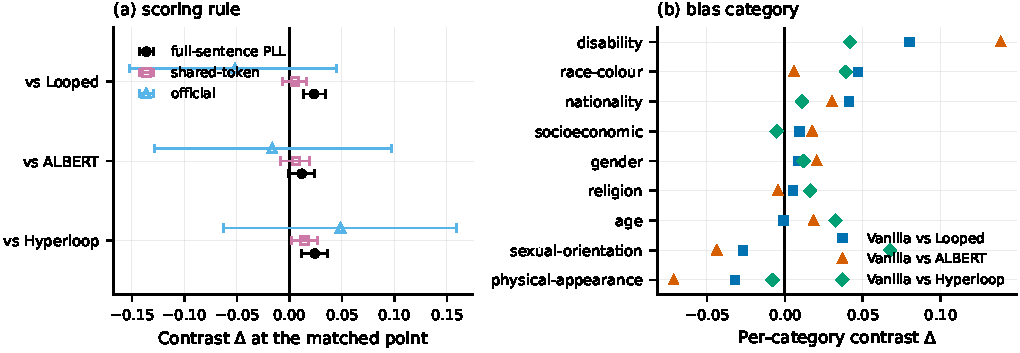
\includegraphics[width=\textwidth]{images/fig4_scorer_and_category.pdf}
\Description{Two panels. Panel a compares the architecture contrast at the
matched point under the full-sentence and changed-token scoring formulations,
with the changed-token intervals crossing zero for two of three contrasts. Panel
b plots the per-category contrast for nine bias categories, showing values on
both sides of zero.}
\caption{Robustness of the architecture contrast. (a) The same comparisons under
the two scoring formulations at the matched point. (b) Per-category contrasts,
ordered by the baseline-versus-looped value; several categories change sign
between architectures.}
\label{fig:robust}
\end{figure*}

\subsection{Category heterogeneity}
\label{sec:category}

The benchmark spans nine bias categories, and the aggregate hides how differently
they behave. Figure~\ref{fig:robust}(b) plots the per-category contrast. Of the
27 category-by-contrast tests, four remain significant after Holm correction
within each contrast, and four of the nine categories change sign depending on
which shared encoder is compared. The aggregate difference is carried mainly by
race-colour, the largest category with 516 items, where the
baseline-versus-looped contrast is 0.0468 ($p_{\text{Holm}} = 0.0009$), and by
disability, a much smaller category of 60 items, where it is 0.0802
($p_{\text{Holm}} = 0.047$). Sexual orientation runs the other way for two of the
three comparisons. These category analyses are descriptive: they were run after
the aggregate instability was found and are not confirmatory tests of a stated
hypothesis.

\subsection{Equivalence of the two looped variants}

The two looped variants differ by 0.00045 at the matched point ($p = 0.93$),
which is an absence of a detected difference rather than evidence of similarity.
A two one-sided tests procedure against a margin of $\pm 0.0118$, half the
observed baseline-versus-looped difference, rejects the presence of a difference
larger than that margin ($p = 0.023$; 90\% interval $[-0.0090, 0.0099]$). The
margin was chosen after the contrast had been examined, so this is an exploratory
equivalence analysis and not a pre-specified one. Read with that caveat, the
extra streams and mixing matrices show no association benefit over plain looping
at this point, while adding 19 million parameters.

\subsection{The capability gate is not met}
\label{sec:capability}

On the coreference instrument all four encoders answer at chance. Jeffreys
intervals over the 374 evaluated items include 0.5 for every architecture and
both splits, with pro-stereotype accuracy between 0.489 and 0.503. A model that
cannot resolve the pronoun cannot show a stereotypical preference in resolving
it, so this leg returns no evidence in either direction. The GLUE leg was not
completed; because the coreference leg already fails, running it could not make
the gate pass, and the compute was not spent. The baseline-interval leg is met,
as Table~\ref{tab:band} shows.

The consequence is that every measurement in this paper indexes association in
the masked language modelling head. None of it demonstrates that a downstream
ranker or classifier built on these encoders would treat groups differently.

\subsection{Optimisation behaviour in these runs}
\label{sec:stability}

In these runs HyperloopBERT was markedly harder to optimise. At the peak learning
rate that trained the other three encoders without incident its validation loss
rose from 2.53 to 6.86 within one interval and then became non-finite; at half
that rate it trained past the earlier failure point and then became non-finite
again. ALBERTLoopedBERT showed one transient spike that recovered within a
thousand steps. With one seed per architecture these are observations about the
runs performed, not evidence of a general property of weight reuse, and no causal
claim is made from them. The snapshots analysed above predate both HyperloopBERT
failures and were checked to contain no non-finite values.

% ================================================================= discussion
\section{Discussion}

\paragraph{Why the single-point result looked convincing.}
Table~\ref{tab:band} has every feature of a solid finding: a pre-stated contrast
set, a paired test on 1508 items, correction for multiplicity, and two of three
comparisons surviving at $p_{\text{Holm}} = 0.0003$. Nothing about it is wrong.
It is simply one draw from a family of equally defensible analyses, and the rest
of that family does not agree with it.

\paragraph{What the all-band view changes.}
Repeating the comparison at every matched point converts a point estimate into a
distribution, and that distribution straddles zero
(Figure~\ref{fig:delta}). The continuous adjustment in Section~\ref{sec:cont}
gives the same answer from a different direction: with realised loss in the
model, the architecture terms are indistinguishable from zero while the loss term
is not. Between the two, capability is doing the work that the architecture
appeared to be doing.

\paragraph{Why two scoring formulations disagree.}
The full-sentence formulation lets the shared context contribute to both members
of the pair; the changed-token formulation removes it by construction. When the
demographic term is a small part of a long sentence, the first is dominated by
context the pair has in common, which raises sensitivity to length and fluency
differences and lowers it to the substitution itself. That the two orderings
agree only at $\rho \approx 0.47$ shows the choice is not cosmetic. Neither is
wrong; a comparison that survives only one of them is not yet a finding.

\paragraph{What iso-loss matching does and does not solve.}
It removes gross differences in training progress, which is a real improvement
over comparing at a fixed token budget. It does not make two checkpoints
interchangeable. The residual gaps here are small in nats, yet the contrast moves
substantially across them, so the sensitivity of the conclusion to the matched
point is larger than the sensitivity of the matching itself.

\paragraph{Category structure.}
An aggregate stereotype score is a mean over categories that do not behave alike,
and here four of nine change sign depending on the comparison. Reporting the
aggregate alone can therefore describe a model as less stereotyping overall while
the pattern reverses within particular categories, which is precisely the
information a practitioner deciding where a system may cause harm would need.

\paragraph{Implication for architecture fairness comparisons.}
Retrieval and classification pipelines routinely choose one pre-trained encoder
over another, and such choices are sometimes justified partly on fairness
grounds. The evidence here is that a comparison of this kind can reverse under
choices that are rarely reported: which matched capability level is used and how
the benchmark is scored. A defensible protocol reports the contrast across
several matched capability levels and at least two scoring formulations, and
treats a result that appears at one operating point only as provisional.

% ================================================================ limitations
\section{Limitations}
\label{sec:limits}

Training uses one seed per architecture. All intervals reported are bootstraps
over benchmark items and describe item sampling, not variation between training
runs, so the ordering of the encoders may not be stable under re-training. This
is the single largest limitation of the study.

The all-band, continuous-adjustment, scorer, category and equivalence analyses
were performed after the single-point result had been examined. They are
robustness checks and are reported as exploratory. Only the three
baseline-versus-shared contrasts at the deepest matched point were specified
before analysis of that point.

The encoders reach roughly two nats at the deepest matched point, well short of a
fully trained model, and the effect size is still changing there for three of the
four (Spearman $\rho = -0.90$, $-0.80$ and $-0.71$; the looped encoder does not
follow the same trend at $\rho = +0.30$). Whether the picture is different for
fully trained encoders is untested.

The measurement is of the correlation type in the sense of
\citet{wang2025difference} and the capability gate is not met, so no statement
about downstream behaviour is supported. The benchmark itself carries documented
item-quality problems \citep{blodgett2021salmon}, of which the eight unalignable
pairs in Section~\ref{sec:scorer} are a concrete instance.

The evaluation is English-only. An India-centric instrument covering caste and
religion \citep{khandelwal2023indianbhed} was planned, but the mirror available
at the time could not be used with an English-only tokeniser. Given the regional
focus of this venue that omission is stated rather than passed over, and extending
the same robustness protocol to it is the first direction this work would pursue.

% =========================================================== reproducibility
\section{Reproducibility}

The corpus is FineWeb-Edu \citep{penedo2024fineweb}, pre-tokenised to fixed-size
blocks with a tokeniser fitted once; a checksum and block-count manifest is
verified at the start of every run. Architectures are as in Table~\ref{tab:arch},
trained with AdamW, peak learning rate $3 \times 10^{-4}$ (HyperloopBERT
$1.5 \times 10^{-4}$), batch size 512, 10\% warmup, gradient clipping 1.0,
bfloat16 autocast, one seed (42), on one H100 GPU. Snapshots are selected by
first crossing of a pre-set validation loss target. Scoring is 32-bit for both
formulations. Tests are sign-flip permutation with $10^4$ draws and
$(b+1)/(m+1)$ $p$-values \citep{phipson2010permutation}, $10^4$-resample item
bootstraps, Holm correction within each contrast family, and cluster-robust OLS
with items as clusters. Analyses run under Python 3.10 with NumPy 2.2, pandas
2.3, SciPy 1.15 and statsmodels 0.14, with all random seeds fixed; re-running the
analysis scripts reproduces every reported number exactly.
% CAMERA-READY: restore the concrete repository and checkpoint URLs here.
Code, per-item scores for every snapshot, and the analysis scripts are available
in an anonymised archive for review.

% ========================================================== GenAI disclosure
\section*{Generative AI Use Disclosure}

In accordance with the ACM policy on generative AI, the authors disclose that a
large language model based coding assistant was used during this work for
software engineering and analysis support: writing and debugging training,
evaluation and statistical-analysis code; generating figures from committed
result files; and copy-editing prose. It was also used to help identify the
robustness weaknesses of an earlier version of this analysis, which prompted the
all-band and scoring-formulation experiments reported here. All experimental
design decisions, all interpretations, and every numerical claim were verified by
the authors against committed outputs. The tool is not an author and bears no
responsibility for the content.

% ================================================================= conclusion
\section{Conclusion}

Four encoders differing in cross-depth weight sharing were pre-trained on
identical data and compared at matched validation loss. At the deepest matched
point two of three shared encoders record a lower stereotype effect than the
unshared baseline. That result does not survive the checks that follow: it
reverses sign across other matched points, disappears once realised loss is
adjusted for continuously, and does not survive correction under the benchmark's
changed-token scoring formulation. The two looped variants are equivalent within
an exploratory margin, aggregate scores conceal category-level sign changes, and
all four encoders answer at chance on a coreference instrument.

The practical conclusion is about method rather than architecture. A bias
comparison between neural architectures that rests on one capability-matched
checkpoint and one scoring definition can reverse under either choice, so such
comparisons should report sensitivity across both before a difference is
attributed to architecture.

\bibliographystyle{ACM-Reference-Format}
\bibliography{reference}

\end{document}
